\chapter{File System}
\label{chp:fs}

\section{Introduction}
\index{Block}
\begin{defn}
	\textbf{Block :} It is the basic unit of storage in the disk.
\end{defn}
	
The disk can be thought of as consisting of a linear sequence of 512 blocks.
The size of each block is equal to that of a page in the memory (256 words). 

\section{Disk Structure}
\index{Disk!Structure}
The basic structure of the disk is shown in figure~\ref{fig:disk}.

\begin{figure}[htp!] \small
	\centering
	\begin{tabular}{|c||c|c|c|c|c|c|c|c|c|}
		\hline
		\textbf{Block No.} & 0 & 1 & 2 & \ldots & 8 & 9--10 & 11--12 & 13--16 & 17--511 \\ \hline
		\textbf{Contents} & OS Startup code & INT 0 & INT 1 & \ldots & INT 7 & Free List & FAT & INIT & Data Blocks \\ \hline
	\end{tabular}
	\caption{Structure of the disk}
	\label{fig:disk}
\end{figure}

\section{Addressing}
\index{Disk!Addressing}
\begin{defn}	
	\textbf{Block number :} Any particular block in the disk is addressed by the corresponding number in the sequence 0 to 511 known as the \emph{block number}.
\end{defn}

\begin{figure}[htp!] 
	\centering
	\scalebox{0.85}{
	\begin{tabular}{|c|c|c|}
		\toprule
		\textbf{Block} & \textbf{Contents} & \textbf{Block no.} \\ \toprule
		\multirow{4}{*}{$1$} & $0^{th}$ word & \multirow{4}{*}{$0$} \\
					  &  $1^{st}$ word &  \\
					  &  \vdots &   \\
					  &  $255^{th}$ word &  \\ \hline
		\multirow{4}{*}{$2$} &  $256^{th}$ word &  \multirow{4}{*}{$1$} \\
					  &  $257^{th}$ word &   \\
					  &  \vdots &  \\
					  &  $511^{th}$ word &  \\ \hline
		\vdots & \vdots & \vdots \\ \hline
		\multirow{3}{*}{$512$} & \vdots & \multirow{3}{*}{511}   \\
					    & \vdots &  \\
					    &  $(256 \times 512 - 1)^{th}$ word &  \\ \bottomrule
	\end{tabular}}
	\caption{Disk addressing}
	\label{fig:disk addr}
\end{figure}

\begin{example}
	In figure~\ref{fig:disk addr}, the $2^{nd}$ block of the disk has a block number 1. In general the $i^{th}$ block has the block number $(i-1)$ for $1 \le n \le 512$. 
\end{example}

\section{Disk Free List}
\index{Disk Free List}
\label{lbl:disklst}
\begin{itemize}
	\item  The Free List of the disk consists of 512 entries. Each entry is of size one word.
	\item  The total size of the free list is thus 2 blocks or 512 words (512(= no. of entries) $\times$ 1(= size of one entry) = 512 words).
	\item  It is present in blocks 9 and 10 of the disk. Refer figure~\ref{fig:disk}. \index{Disk!Free List Location}
	\item  Each entry of the free list contains a value of either 0 or 1 indicating whether the corresponding block in the disk is free or not respectively (It should be ensured that the first 13 entries are always marked used).
\end{itemize}
\begin{example}
	Figure~\ref{fig:disk free list} indicates that the blocks 0, 1 and 511 of the disk are not free while blocks 2 and 48 are free.
\end{example}

\begin{figure}[htp!] \small
	\centering
	\begin{tabular}{|c|c|}
		\multicolumn{2}{c}{} \\ \toprule
		\textbf{Index} & \textbf{Content} \\ \toprule
		$0$ & $1$ \\ \hline
		$1$ & $1$ \\ \hline
		$2$ & $0$ \\ \hline
		\vdots & \vdots \\ \hline
		$48$ & $0$ \\ \hline
		$\vdots$ & \vdots \\ \hline
		$511$ & $1$ \\ \hline
	\end{tabular}
	\caption{A sample free list of the disk}
	\label{fig:disk free list}
\end{figure}

\section{File}
A file \index{File} is a collection of data identified by a name. Every file in the disk has a \textit{Basic Block} and several \textit{Data Blocks}. They are defined as follows:
\begin{itemize}
	\item \textbf{Data Blocks :}  These blocks contain the actual data of a file. \index{File!Data Block}
	\item \textbf{Basic Block :}  It consists of information about the data of a file. \index{File!Basic Block}
% 	 	the location of the data blocks of the file in the disk etc.  	
	\begin{itemize}
		\item The basic block structure is shown in figure~\ref{fig:basic block}. \index{File!Basic Block Structure}
		\begin{figure}[h]
			\centering
			\begin{tabular}{|c|c|c|}
				\hline
				\textbf{Index} & 0--127 & 128--255\\
				\hline
				\textbf{Content} & Block List & Header\\
				\hline
			\end{tabular}
			\caption{Structure of the basic block of a file}
			\label{fig:basic block}
		\end{figure}
		\item The basic block consists of the \textit{Block List} and the \textit{Header}.
		\item \textbf{Block List :} It is similar to an index in a book which tells which chapter starts from which page.
		\begin{itemize}
			\item The block list consists of 128 entries.
			\item Each entry is of size one word.
			\item The size of the block list is thus 128 words (128(= no. of entries) x 1(= size of an entry) = 128 words).
			\item The value contained in an entry of the block list gives the block number of the corresponding data block in the disk.
		\end{itemize}
		\item \textbf{Header :} The header contains the header information relating to the file. Currently this is unused, but at a later stage can be used to store information such as file modification date/time, author of the file etc.
	\end{itemize}
\end{itemize}

\begin{example}
	\begin{figure}[h!]
	\centering
	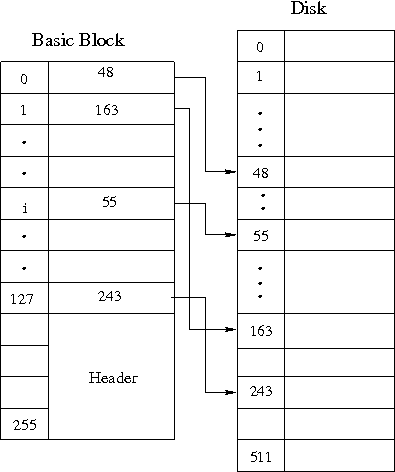
\includegraphics[scale=0.60]{pics/basic_block_example}
	\caption{Example illustrating the basic block of a file}
	\label{basic block example}
	\end{figure}

	Consider the example illustrated by figure~\ref{basic block example}.
	From the figure, we infer the following. 
	\begin{itemize}
		\item  The zeroth data block of the file resides at the disk block whose block number is 48. 
		\item  The first data block of the file resides at the disk block whose block number is 163.
		\item  The ith data block of the file resides at the disk block whose block number is 55 where $ 0\le i \le 127$. 
		\item  The 127th data block of the file resides at the disk block whose block number is 243.
	\end{itemize}
\end{example}

\subsection{File Types} 
\index{File!Types}
There are two types of files in the \ESIM architecture. They are:
\begin{enumerate}
	\item \textbf{Data files :} These files contain data or information that is used by the programs. They can occupy a maximum of 129 blocks (1 basic block + 0 - 128 data blocks).
	\item \textbf{Executable files :} These contain programs that the user wishes to run on the machine. They occupy 4 blocks (1 basic block + 3 data blocks) of the disk.
\end{enumerate}


\subsection{Executable File Format}
\index{Executable File Format}
Any executable file has the following format. Refer figure~\ref{fig:executable}.
\begin{itemize}
	\item  It consists of the \emph{Code section} and the \emph{Data section}.
	\item \textbf{Code section :} This section contains the actual code to be run on the machine. It spans 2 blocks irrespective of the size of the code.
	\index{Executable File Format!Code Section}
	\item \textbf{Data Section :} This section consists of data that is used in the code which cannot be stored in a register. The registers then store the logical address of the corresponding data residing in the data section. It spans 1 block. \index{Executable File Format!Data Section}
\end{itemize}
	
\begin{figure}[h!]
	\centering
	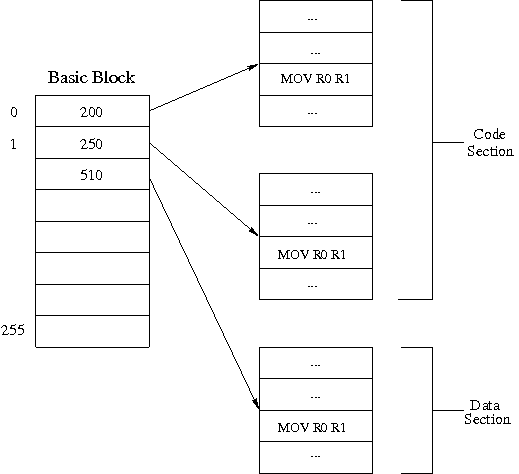
\includegraphics[scale=0.60]{pics/executable}
	\caption{Example illustrating the structure of an executable in the disk}
	\label{fig:executable}
\end{figure}

\section{File Allocation Table (FAT)}
\index{File Allocation Table}
\label{sec:fat}
\label{lbl:fat}
\emph{File allocation table} (FAT), as the name suggests, is a table that has an entry for each file present in the disk.
\begin{itemize}
	\item FAT of the filesystem consists of 32 entries. Thus there can be a maximum of 32 files. 
	\item Each entry is of size 16 words.
	\item Total size of the FAT is thus 512 words (32 (= number of entries) $\times$ 16(= size of one entry) = 512 words).
	\item It is a disk data structure and occupies block numbers 11 and 12 of the disk. Refer figure~\ref{fig:disk}. 
	\index{File Allocation Table!Location in disk}
\end{itemize}

The structure of a FAT entry is shown in figure~\ref{fig:fat_entry}. 

\begin{figure}[htp!] \small
	\centering
	\begin{tabular}{|c|c|c|c|}
		\hline
		0 & 1 & 2 & 3 -- 15 \\
		\hline
		File Name & File Size & Block no: of basic block & \dots{} Free \dots \\
		\hline
	\end{tabular}
	\caption{Structure of a FAT entry}
	\label{fig:fat_entry}
\end{figure}

The FAT entry consists of the
\index{File Allocation Table!FAT Entry}
\begin{enumerate}
	\item \textbf{File Name :} It is an identification of a file. It can be of maximum 15 characters (and thus requires 1 word). Typical file names are \texttt{student.txt}, \texttt{calc.sim}.
	\item \textbf{File size :} It indicates the number of words occupied by a file. It varies from 0 words to (128 $\times$ 256) words (depending upon the number of data blocks it has). It occupies one word in the FAT entry.
	\item \textbf{Block number of basic block :} It contains the block number where the basic block of a file resides in the disk. It occupies one word in the FAT entry.
\end{enumerate}

% \section{Restrictions}
